\chapter{Incertidumbre, teorema de Ehrenfest y límite clásico}

\section{El cabo suelto del Hamiltoniano lineal}

El modelo
\begin{equation}
H=cP
\label{eq:l10-linear-hamiltonian}
\end{equation}
era útil porque sus paquetes de onda se trasladan sin cambiar de forma. También encierra una advertencia seria. El momento puede ser positivo o negativo, por lo que la misma fórmula asigna energía positiva a una onda plana y energía negativa a la otra:
\begin{equation}
\psi_p(x)=e^{ipx/\hbar},
\qquad
E(p)=cp.
\end{equation}
Si un número arbitrariamente grande de partículas físicas pudiera ocupar estados de energía negativa, el espacio vacío no sería el estado de menor energía. Podría producir cuantos de energía positiva mientras deposita energía negativa compensatoria en partículas nuevas, conservando la energía total pero haciendo que la energía del vacío disminuyera sin límite.

\begin{classroomqa}
\audiencequestion{¿Por qué una rama de energía negativa es algo más que una elección extraña del cero de energía?}
\lecturerresponse{Un desplazamiento aditivo común de todas las energías no plantea ningún problema. Un espectro no acotado es distinto. Si se pueden poblar estados de energía cada vez menor mientras partículas de energía positiva se llevan el balance, no existe un estado fundamental estable. La estabilidad exige que la energía esté acotada inferiormente con respecto al vacío.}
\end{classroomqa}

\begin{figure}[htbp]
\centering
\includegraphics[width=0.88\textwidth]{lecture_10_figure_01.png}
\caption{El Hamiltoniano lineal y sus funciones propias de onda plana muestran la rama de energía negativa cuando \(p<0\).}
\lectureframe{00:04:35}
\end{figure}

La respuesta histórica de Dirac funcionaba para los fermiones. Los fermiones obedecen el principio de exclusión: dos fermiones idénticos no pueden ocupar el mismo estado de una partícula. Imaginemos que se llena cada estado de energía negativa. Una vez ocupados todos, la exclusión impide que otro fermión caiga en ese sector. Un estado vacante en el conjunto lleno se comporta como una antipartícula.

Este argumento no resuelve el problema de los bosones de energía negativa. Cualquier número de bosones puede ocupar un mismo estado, así que un modo bosónico de energía negativa podría poblarse sin límite. Conviene considerar la antigua imagen del mar lleno como la vía histórica que condujo a las antipartículas; la teoría cuántica de campos moderna organiza las partículas y las antipartículas sin tratar el vacío físico como un mar literal de electrones observables de energía negativa. Aquí solo necesitamos una conclusión más acotada: el Hamiltoniano de juguete no constituye una teoría completa y estable de partículas.

Como caricatura unidimensional de una partícula fermiónica que se mueve a velocidad constante, el modelo apunta al problema del neutrino al que eran pertinentes las ideas de Dirac. No puede servir como teoría del fotón: los fotones son bosones y el principio de exclusión no puede llenar y bloquear sus estados de energía negativa.

\begin{classroomqa}
\audiencequestion{¿Por qué la exclusión puede estabilizar la construcción fermiónica, pero no una bosónica?}
\lecturerresponse{Un estado fermiónico puede llenarse una vez y quedar entonces bloqueado. Un estado bosónico no tiene ese límite de ocupación, de modo que un modo bosónico de energía negativa seguiría permitiendo que la energía disminuyera sin límite.}
\end{classroomqa}

\paragraph{Situación actual del curso.}
Este trimestre ha desarrollado buena parte de los fundamentos de la mecánica cuántica y varios sistemas deliberadamente sencillos, pero muy pocas aplicaciones. En particular, aún no ha llegado ni siquiera al oscilador armónico. Esa omisión marca un límite, no un final: a continuación vienen la relatividad y la teoría de campos, tras lo cual habrá que retomar la mecánica cuántica para estudiar el oscilador y las demás estructuras que se basan en él. El interés sostenido por la discusión anterior sobre el entrelazamiento también muestra por qué valió la pena seguir esta ruta hacia los fundamentos.

Con esa perspectiva, cerramos el cabo suelto. El tema central es la función de onda, la incertidumbre y la relación entre la evolución cuántica y la mecánica clásica. El objetivo no es la ecuación de evolución más general posible, sino la ecuación particular en la representación de posición que escribió originalmente Schr\"odinger.

\section{Funciones de onda y coordenadas completas que conmutan}

Para una partícula en una recta, la función de onda en la representación de posición es
\begin{equation}
\psi(x)=\braket{x}{\psi},
\end{equation}
la amplitud de probabilidad de encontrar la partícula cerca de \(x\). La función de onda en la representación de momento es
\begin{equation}
\widetilde{\psi}(p)=\braket{p}{\psi}.
\end{equation}
Describen el mismo estado abstracto en bases distintas y están relacionadas por una transformada de Fourier:
\begin{align}
\psi(x)
&=
\int_{-\infty}^{\infty}
\frac{dp}{\sqrt{2\pi\hbar}}\,
\widetilde{\psi}(p)e^{ipx/\hbar},
\label{eq:l10-fourier-forward}\\
\widetilde{\psi}(p)
&=
\int_{-\infty}^{\infty}
\frac{dx}{\sqrt{2\pi\hbar}}\,
\psi(x)e^{-ipx/\hbar}.
\label{eq:l10-fourier-inverse}
\end{align}

\begin{figure}[htbp]
\centering
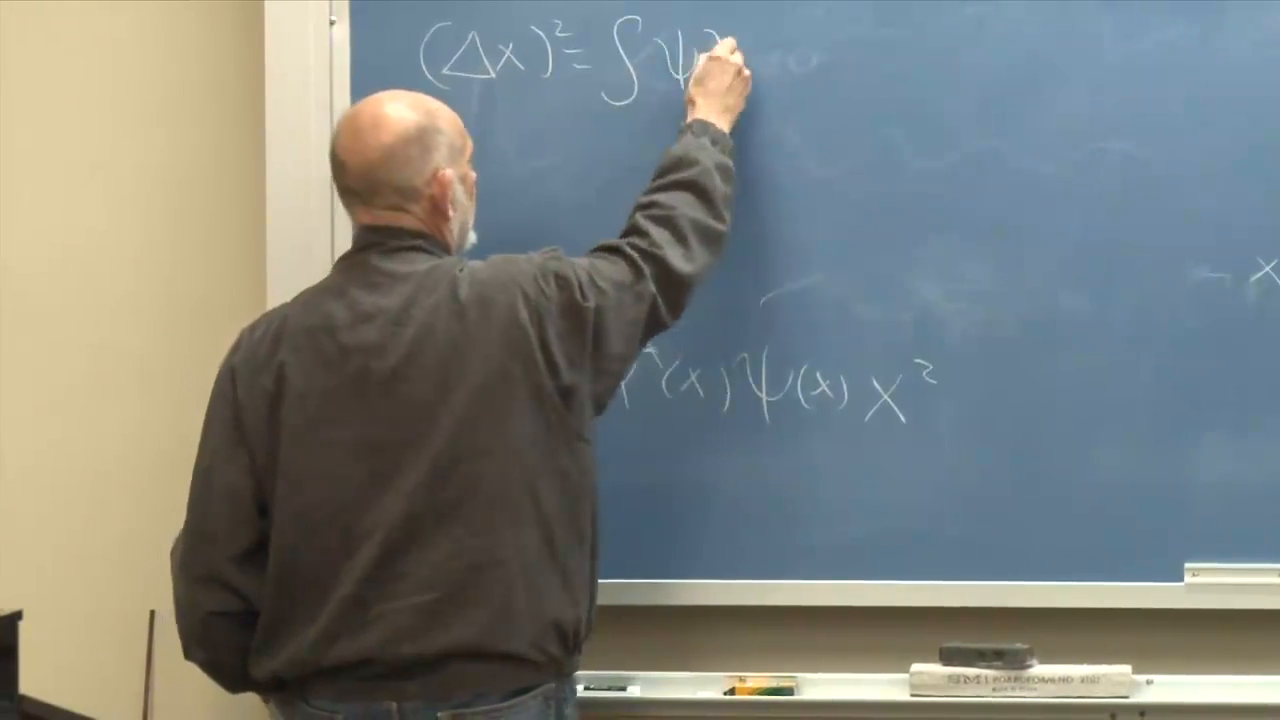
\includegraphics[width=0.88\textwidth]{lecture_10_figure_02.png}
\caption{Las funciones de onda en las representaciones de posición y de momento son proyecciones de un mismo estado sobre dos bases continuas distintas.}
\lectureframe{00:09:05}
\end{figure}

En dos dimensiones espaciales, \(X\) y \(Y\) conmutan, por lo que una base propia común puede etiquetarse con ambas coordenadas y la función de onda pasa a ser \(\psi(x,y)\). Esa conmutación no se deduce únicamente de los axiomas abstractos; forma parte de la descripción cuántica de nuestro espacio ordinario, confirmada empíricamente. Para \(N\) partículas en tres dimensiones,
\begin{equation}
\psi(\mathbf{x}_1,\ldots,\mathbf{x}_N)
\end{equation}
es una función en el espacio de configuraciones, no una onda tridimensional independiente asociada por separado a cada partícula. Por tanto, un sistema macroscópico puede requerir un número enorme de coordenadas.

\begin{classroomqa}
\audiencequestion{¿La conmutación de distintas coordenadas espaciales se deduce automáticamente de la mecánica cuántica?}
\lecturerresponse{No. El marco abstracto admite muchas álgebras de observables. El hecho de que distintas componentes cartesianas de la posición conmuten es un hecho estructural empírico de la mecánica cuántica de las partículas en el espacio ordinario.}
\end{classroomqa}

Se puede aplicar una transformada de Fourier a cada coordenada y obtener una función de onda de todos los momentos, o transformar solo algunas variables. Las representaciones mixtas son legítimas porque una representación es una elección de base, no un cambio del estado físico.

\section{Qué mide la incertidumbre}

La forma más elemental del principio de incertidumbre se deduce de inmediato del par de Fourier. Un estado de momento definido es una onda plana de módulo constante, sin localización en posición. Un estado bien localizado en posición requiere muchas componentes de momento. En general, al estrecharse una de las funciones de un par de Fourier, la otra se ensancha.

\begin{figure}[htbp]
\centering
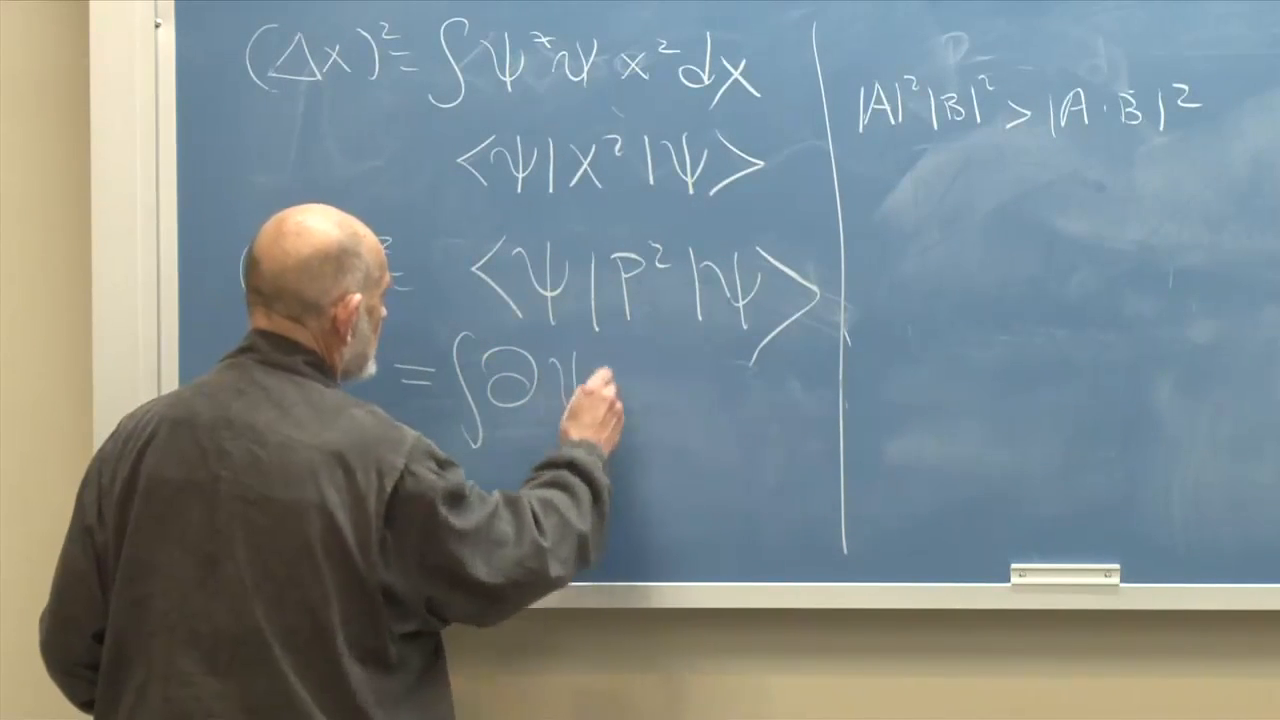
\includegraphics[width=0.88\textwidth]{lecture_10_figure_03.png}
\caption{Un perfil de posición localizado requiere una superposición amplia de ondas planas en la representación recíproca del momento.}
\lectureframe{00:14:45}
\end{figure}

Para expresar esta afirmación cuantitativamente, empecemos con un observable general \(Q\). Su valor esperado en un estado normalizado es
\begin{equation}
\expect{Q}=\bra{\psi}Q\ket{\psi}.
\end{equation}
La varianza es
\begin{equation}
(\Delta Q)^2
=
\expect{\bigl(Q-\expect{Q}\bigr)^2}
=
\expect{Q^2}-\expect{Q}^2.
\label{eq:l10-general-variance}
\end{equation}
La incertidumbre \(\Delta Q\) es la raíz cuadrada positiva de esta varianza.

Para la posición, primero podemos desplazar el origen de modo que \(\expect{X}=0\). Entonces,
\begin{equation}
(\Delta x)^2
=
\expect{X^2}
=
\int_{-\infty}^{\infty}
dx\,|\psi(x)|^2x^2.
\label{eq:l10-position-variance}
\end{equation}
Las contribuciones positivas y negativas se cancelan en \(\expect{X}\), pero se suman en \(\expect{X^2}\). Por tanto, una distribución de probabilidad más ancha tiene una varianza mayor.

\begin{figure}[htbp]
\centering
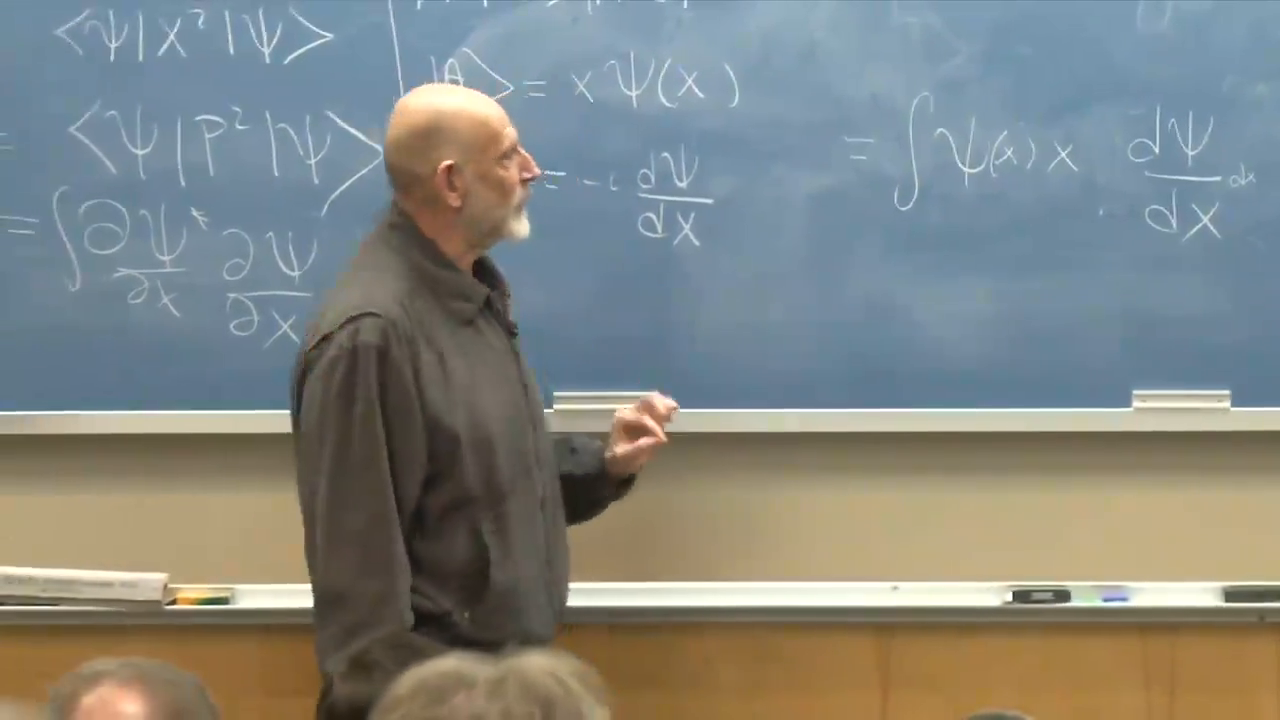
\includegraphics[width=0.88\textwidth]{lecture_10_figure_04.png}
\caption{Con la media desplazada a cero, la varianza de la posición es la integral de \(x^2\) ponderada por la probabilidad.}
\lectureframe{00:20:50}
\end{figure}

La distinción entre \(\expect{X^2}\) y \(\expect{X}^2\) es esencial. Una distribución simétrica respecto de cero tiene \(\expect{X}=0\), pero, a menos que esté concentrada en el origen, también tiene \(\expect{X^2}>0\).

La varianza del momento puede definirse directamente en el espacio de momentos:
\begin{equation}
(\Delta p)^2
=
\int_{-\infty}^{\infty}
dp\,|\widetilde{\psi}(p)|^2
\bigl(p-\expect{P}\bigr)^2.
\end{equation}
Para la demostración resulta más útil trabajar en el espacio de posiciones. Desplacemos la media del momento a cero y usemos
\begin{equation}
P=-i\hbar\frac{d}{dx},
\qquad
P^2=-\hbar^2\frac{d^2}{dx^2}.
\end{equation}
Entonces,
\begin{equation}
(\Delta p)^2
=
\expect{P^2}
=
-\hbar^2
\int_{-\infty}^{\infty}
dx\,\psi^*(x)\frac{d^2\psi}{dx^2}.
\label{eq:l10-momentum-variance-second}
\end{equation}

\begin{classroomqa}
\audiencequestion{¿Cómo puede ser positiva una varianza si su expresión en el espacio de posiciones comienza con un signo menos?}
\lecturerresponse{La integral que multiplica ese signo es no positiva. Al integrar por partes, se transfiere una derivada a \(\psi^*\), aparece un segundo signo menos y el resultado se convierte en la integral de un módulo al cuadrado.}
\end{classroomqa}

Para funciones de onda que decrecen suficientemente rápido en el infinito,
\begin{equation}
\int f\,g'\,dx
=
\left[fg\right]_{-\infty}^{\infty}
-
\int f'g\,dx,
\end{equation}
y el término de borde se anula. Al aplicar esto una vez a la ecuación~\eqref{eq:l10-momentum-variance-second}, se obtiene
\begin{equation}
(\Delta p)^2
=
\hbar^2
\int_{-\infty}^{\infty}
dx\,
\frac{d\psi^*}{dx}
\frac{d\psi}{dx}
=
\hbar^2
\int_{-\infty}^{\infty}
dx\,
\left|\frac{d\psi}{dx}\right|^2
\geq 0.
\label{eq:l10-momentum-variance-positive}
\end{equation}

\begin{figure}[htbp]
\centering
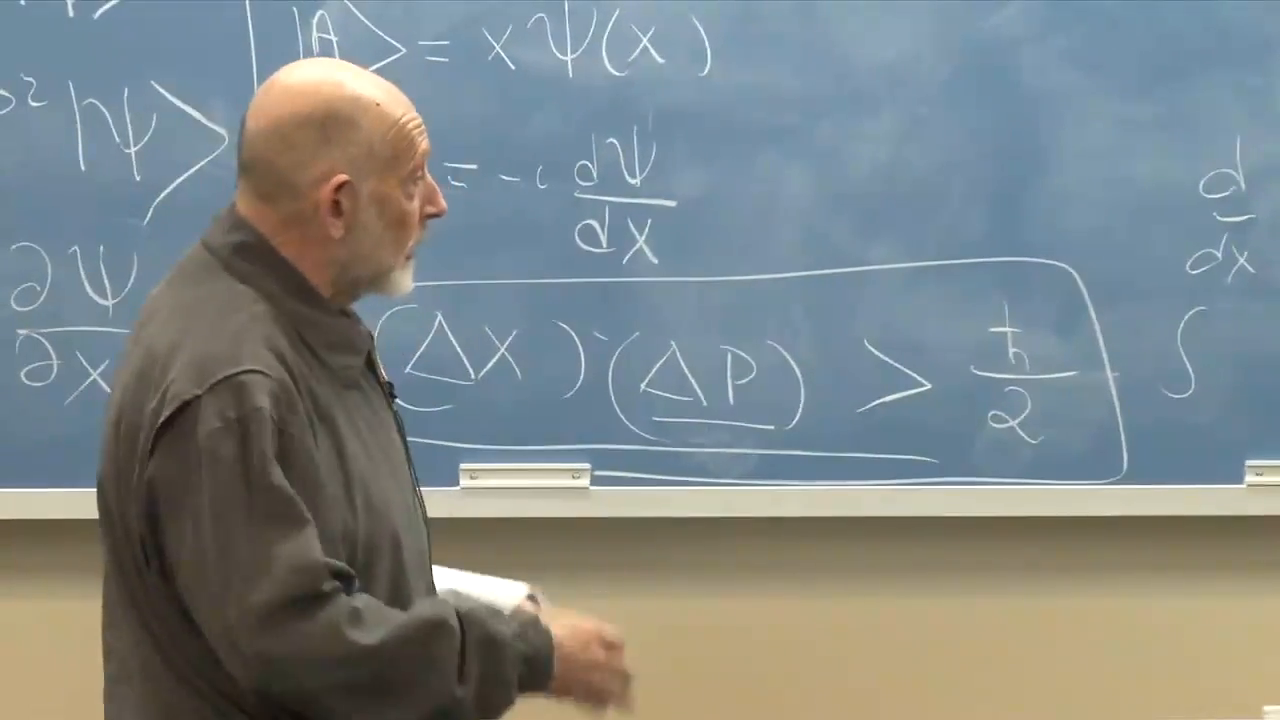
\includegraphics[width=0.88\textwidth]{lecture_10_figure_05.png}
\caption{La integración por partes transforma la expresión aparentemente negativa de \(\expect{P^2}\) en una norma manifiestamente positiva.}
\lectureframe{00:27:35}
\end{figure}

\begin{classroomqa}
\audiencequestion{¿Se pueden desplazar simultáneamente a cero las medias de posición y de momento?}
\lecturerresponse{Sí. Trasladar el argumento de la función de onda desplaza \(\expect{X}\), mientras que multiplicarla por una fase de onda plana desplaza \(\expect{P}\). Estas operaciones modifican las medias sin alterar las varianzas correspondientes, así que en la demostración se pueden usar ambas variables centradas.}
\end{classroomqa}

\section{La cota de incertidumbre}

La herramienta matemática que necesitamos es la desigualdad de Cauchy--Schwarz. La clase la introduce mediante geometría vectorial elemental: el producto escalar de dos vectores es el producto de sus longitudes por el coseno del ángulo que forman, así que su módulo no puede superar el producto de sus longitudes. En la notación de espacios de Hilbert,
\begin{equation}
\braket{A}{A}\braket{B}{B}
\geq
\left|\braket{A}{B}\right|^2.
\label{eq:l10-cauchy-schwarz}
\end{equation}
Se cumple en espacios vectoriales reales o complejos de cualquier dimensión.

\begin{figure}[htbp]
\centering
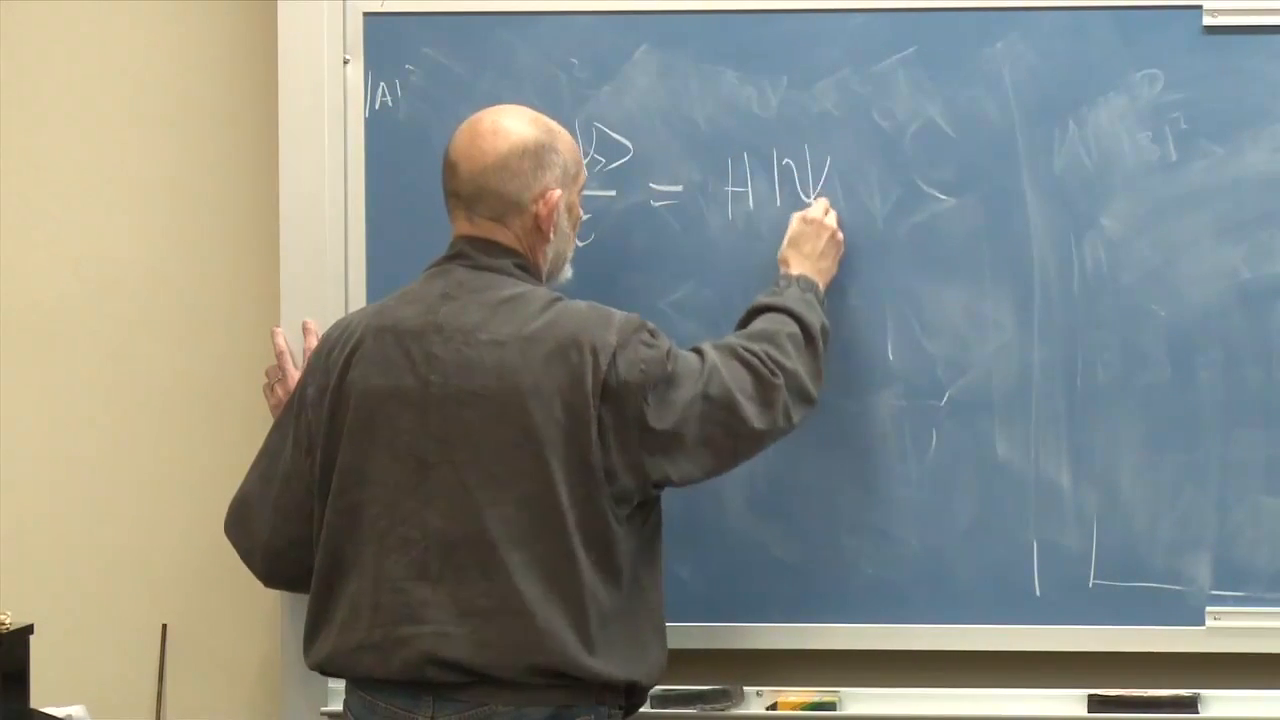
\includegraphics[width=0.88\textwidth]{lecture_10_figure_06.png}
\caption{La desigualdad geométrica para vectores se reformula como la cota de Cauchy--Schwarz en el espacio de Hilbert que se usa en la demostración.}
\lectureframe{00:35:35}
\end{figure}

\begin{classroomqa}
\audiencequestion{¿La desigualdad debe ser estricta o puede darse la igualdad?}
\lecturerresponse{Es una relación de mayor o igual. Se da la igualdad cuando los dos vectores del espacio de Hilbert son linealmente dependientes. Más adelante, esa condición de igualdad permitirá identificar los paquetes de onda de incertidumbre mínima.}
\end{classroomqa}

Centremos ambas variables y sigamos primero la demostración simplificada de la pizarra, que supone que \(\psi(x)\) es real. Definamos
\begin{equation}
\ket{A}=X\ket{\psi},
\qquad
\ket{B}=P\ket{\psi}.
\label{eq:l10-auxiliary-vectors}
\end{equation}
Sus normas al cuadrado son precisamente las varianzas:
\begin{equation}
\braket{A}{A}=(\Delta x)^2,
\qquad
\braket{B}{B}=(\Delta p)^2.
\end{equation}

\begin{figure}[htbp]
\centering
\includegraphics[width=0.88\textwidth]{lecture_10_figure_07.png}
\caption{Los vectores auxiliares \(X\ket{\psi}\) y \(P\ket{\psi}\) expresan las dos varianzas como normas en el espacio de Hilbert.}
\lectureframe{00:44:40}
\end{figure}

El producto interno restante es
\begin{align}
\braket{A}{B}
&=
\int_{-\infty}^{\infty}
dx\,
x\psi(x)
\left(-i\hbar\frac{d\psi}{dx}\right).
\end{align}
Solo interviene su módulo. Como \(\psi\) es real,
\begin{equation}
\psi\frac{d\psi}{dx}
=
\frac{1}{2}\frac{d}{dx}\psi^2.
\end{equation}
Por tanto,
\begin{align}
\left|\braket{A}{B}\right|
&=
\frac{\hbar}{2}
\left|
\int_{-\infty}^{\infty}
dx\,
x\frac{d}{dx}\psi^2
\right| \notag\\
&=
\frac{\hbar}{2}
\left|
-\int_{-\infty}^{\infty}
dx\,\psi^2
\right|
=
\frac{\hbar}{2},
\label{eq:l10-inner-product-half-hbar}
\end{align}
donde la integración por partes elimina la derivada de \(\psi^2\), \(d x/dx=1\), el término de borde se anula y la normalización proporciona la última igualdad.

Sustituyamos la ecuación~\eqref{eq:l10-inner-product-half-hbar} en Cauchy--Schwarz:
\begin{equation}
(\Delta x)^2(\Delta p)^2
\geq
\frac{\hbar^2}{4}.
\end{equation}
Al tomar la raíz cuadrada positiva se obtiene
\begin{equation}
\boxed{
\Delta x\,\Delta p
\geq
\frac{\hbar}{2}
}.
\label{eq:l10-uncertainty-principle}
\end{equation}

\begin{figure}[htbp]
\centering
\includegraphics[width=0.88\textwidth]{lecture_10_figure_08.png}
\caption{El paso de integración por partes y la normalización conducen a la cota precisa de incertidumbre entre posición y momento.}
\lectureframe{00:50:55}
\end{figure}

La restricción de que \(\psi\) sea real era una comodidad para la pizarra, no una limitación del teorema. Para un estado complejo general, tomemos
\begin{equation}
\ket{A}=(X-\expect{X})\ket{\psi},
\qquad
\ket{B}=(P-\expect{P})\ket{\psi}.
\end{equation}
El conmutador fija la parte imaginaria de su producto interno:
\begin{equation}
\operatorname{Im}\braket{A}{B}
=
\frac{1}{2i}\expect{[X,P]}
=
\frac{\hbar}{2}.
\end{equation}
Como \(|\braket{A}{B}|\) es al menos tan grande como el módulo de su parte imaginaria, se obtiene la misma cota.

\begin{classroomqa}
\audiencequestion{¿Qué ocurrió exactamente con el término de borde en las sucesivas integraciones por partes?}
\lecturerresponse{Para los paquetes normalizables que consideramos aquí, los productos que aparecen en \(+\infty\) y \(-\infty\) se anulan. En un intervalo periódico finito, los términos de los extremos se cancelan. El dominio de los operadores debe elegirse de modo que estas afirmaciones se cumplan; de lo contrario, la manipulación formal no está justificada.}
\end{classroomqa}

\begin{classroomqa}
\audiencequestion{¿Se puede alcanzar físicamente la igualdad o la cota inferior es solo una estimación?}
\lecturerresponse{Se puede alcanzar. La igualdad en Cauchy--Schwarz exige que los dos vectores auxiliares sean proporcionales. Al resolver esa condición se obtienen paquetes gaussianos, los estados de incertidumbre mínima que veremos a continuación.}
\end{classroomqa}

\section{Otros pares conjugados de Fourier}

La relación de incertidumbre entre tiempo y energía se parece a la que existe entre posición y momento. Sin embargo, requiere más cuidado, porque aquí el tiempo suele ser un parámetro de evolución, no un observable representado por un operador autoadjunto universal. Desarrollemos un estado en vectores propios de la energía:
\begin{equation}
\ket{\psi(t)}
=
\int dE\,
\phi(E)e^{-iEt/\hbar}\ket{E}.
\label{eq:l10-time-energy-fourier}
\end{equation}
Las amplitudes de energía y la variación temporal están relacionadas por Fourier. Una distribución estrecha de energía varía lentamente y no puede producir un pulso con una localización temporal precisa; una distribución amplia de energía puede producir una envolvente breve para el tiempo de llegada.

\begin{figure}[htbp]
\centering
\includegraphics[width=0.88\textwidth]{lecture_10_figure_09.png}
\caption{La dependencia temporal se construye a partir de estados propios de la energía con fases \(e^{-iEt/\hbar}\), que proporcionan la base de Fourier de la relación entre tiempo y energía.}
\lectureframe{00:53:40}
\end{figure}

\begin{classroomqa}
\audiencequestion{¿Se aplica directamente la misma demostración al tiempo y la energía?}
\lecturerresponse{Sí se aplica la intuición de anchuras recíprocas, y un paquete de ondas que pasa ofrece un ejemplo útil: una ventana breve para el tiempo de llegada requiere una distribución amplia de energía. La formulación con operadores es más sutil, porque el tiempo no interviene en esta formulación exactamente como lo hace \(X\).}
\end{classroomqa}

El ángulo y el momento angular forman otro par conjugado para el movimiento de rotación. Localmente, su relación de Fourier se parece a la de posición y momento. Globalmente, la periodicidad del ángulo requiere cuidados adicionales, por lo que aquí se trata de una analogía y no de un teorema completo.

\begin{classroomqa}
\audiencequestion{¿Son ejemplos aislados los pares posición-momento, tiempo-energía y ángulo-momento angular?}
\lecturerresponse{No. Las variables canónicamente conjugadas aparecen una y otra vez como pares de Fourier. Los detalles relativos a los dominios y la periodicidad varían, pero la localización recíproca es la estructura común.}
\end{classroomqa}

\section{La ecuación de Schr\"odinger en la representación de posición}

Volvamos ahora a la dinámica. La ley abstracta es
\begin{equation}
i\hbar\frac{d}{dt}\ket{\psi(t)}
=
H\ket{\psi(t)}.
\label{eq:l10-abstract-schrodinger}
\end{equation}
Para una partícula de masa \(m\) en un potencial \(V(X)\), tomemos
\begin{equation}
H=\frac{P^2}{2m}+V(X).
\label{eq:l10-particle-hamiltonian}
\end{equation}
Esto incorpora la forma clásica de energía cinética más energía potencial y, a continuación, permite comprobar si su evolución cuántica reproduce el movimiento clásico en el régimen adecuado.

\begin{figure}[htbp]
\centering
\includegraphics[width=0.88\textwidth]{lecture_10_figure_10.png}
\caption{El Hamiltoniano actúa sobre el vector de estado abstracto en la ecuación de Schr\"odinger dependiente del tiempo.}
\lectureframe{00:59:05}
\end{figure}

En la representación de posición, \(P^2\) se convierte en una segunda derivada. Una función de \(X\) actúa por multiplicación:
\begin{equation}
\bigl(V(X)\psi\bigr)(x)=V(x)\psi(x).
\end{equation}
En consecuencia,
\begin{equation}
i\hbar\frac{\partial\psi(x,t)}{\partial t}
=
\left[
-\frac{\hbar^2}{2m}\frac{\partial^2}{\partial x^2}
+V(x)
\right]\psi(x,t).
\label{eq:l10-position-schrodinger}
\end{equation}

\begin{figure}[htbp]
\centering
\includegraphics[width=0.88\textwidth]{lecture_10_figure_11.png}
\caption{El Hamiltoniano de la partícula se convierte en la segunda derivada cinética más la multiplicación por \(V(x)\).}
\lectureframe{01:03:05}
\end{figure}

\begin{classroomqa}
\audiencequestion{¿En qué sentido la función ordinaria \(V(x)\) es un operador?}
\lecturerresponse{Una vez elegida una base de posición, \(X\) actúa multiplicando por \(x\). Por tanto, una función suficientemente regular \(V(X)\) actúa multiplicando en cada punto por el número correspondiente \(V(x)\). Su utilidad se comprueba mediante la dinámica que sigue.}
\end{classroomqa}

Para calcular los valores esperados, despejemos de la ecuación~\eqref{eq:l10-position-schrodinger} las dos derivadas temporales:
\begin{align}
\dot{\psi}
&=
\frac{i\hbar}{2m}\psi''
-\frac{i}{\hbar}V\psi,
\label{eq:l10-psi-dot}\\
\dot{\psi}^{\,*}
&=
-\frac{i\hbar}{2m}\psi^{*\,\prime\prime}
+\frac{i}{\hbar}V\psi^*.
\label{eq:l10-psi-star-dot}
\end{align}
La segunda línea no es más que el complejo conjugado de la primera, pero escribir ambas permite ver las cancelaciones.

\section{El movimiento del centro del paquete}

El centro de la distribución de posición es
\begin{equation}
\expect{X}
=
\int_{-\infty}^{\infty}
dx\,\psi^*(x,t)\,x\,\psi(x,t).
\end{equation}
Derivémoslo:
\begin{equation}
\frac{d}{dt}\expect{X}
=
\int dx\,
\left(
\dot{\psi}^{\,*}x\psi
+
\psi^*x\dot{\psi}
\right).
\label{eq:l10-x-expectation-derivative}
\end{equation}
Los dos términos son complejos conjugados. Al sustituir las ecuaciones~\eqref{eq:l10-psi-dot} y \eqref{eq:l10-psi-star-dot}, los términos del potencial se cancelan porque \(V(x)\) es real. Al integrar por partes los términos cinéticos, queda
\begin{align}
\frac{d}{dt}\expect{X}
&=
\frac{1}{m}
\int dx\,
\psi^*
\left(-i\hbar\frac{\partial}{\partial x}\right)
\psi \notag\\
&=
\frac{\expect{P}}{m}.
\label{eq:l10-ehrenfest-x}
\end{align}

\begin{figure}[htbp]
\centering
\includegraphics[width=0.88\textwidth]{lecture_10_figure_12.png}
\caption{La derivada del centro del paquete se reduce al valor esperado del momento dividido por la masa.}
\lectureframe{01:15:40}
\end{figure}

Esta relación es exacta. En el álgebra no se ha usado ninguna aproximación de paquete estrecho.

\begin{classroomqa}
\audiencequestion{¿En qué parte de esta derivación se supuso que el paquete de onda es un único pico estrecho?}
\lecturerresponse{En ninguna. La identidad \(d\expect{X}/dt=\expect{P}/m\) se cumple para todos los estados del dominio de este Hamiltoniano. La localización solo importa cuando interpretamos \(\expect{X}\) como la trayectoria de una partícula clásica.}
\end{classroomqa}

La otra mitad de la mecánica se refiere al momento:
\begin{equation}
\expect{P}
=
\int dx\,
\psi^*
\left(-i\hbar\frac{\partial}{\partial x}\right)
\psi.
\end{equation}
Derivemos los dos factores que dependen del tiempo:
\begin{equation}
\frac{d}{dt}\expect{P}
=
-i\hbar
\int dx\,
\left(
\dot{\psi}^{\,*}\psi'
+
\psi^*\frac{\partial\dot{\psi}}{\partial x}
\right).
\label{eq:l10-p-expectation-start}
\end{equation}
Tras integrar un término por partes, sustituyamos las dos ecuaciones de Schr\"odinger. Las contribuciones cinéticas se cancelan. Los términos del potencial se combinan para dar
\begin{equation}
\int dx\,
V(x)
\left(
\psi\frac{\partial\psi^*}{\partial x}
+
\psi^*\frac{\partial\psi}{\partial x}
\right)
=
\int dx\,
V(x)\frac{\partial}{\partial x}|\psi|^2.
\end{equation}
Una última integración por partes traslada la derivada al potencial:
\begin{align}
\frac{d}{dt}\expect{P}
&=
-\int dx\,|\psi(x,t)|^2\frac{dV}{dx} \notag\\
&=
-\expect{V'(X)}
\\
&=
\expect{F(X)},\\
F(x)&=-V'(x).
\label{eq:l10-ehrenfest-p}
\end{align}

\begin{figure}[htbp]
\centering
\includegraphics[width=0.88\textwidth]{lecture_10_figure_13.png}
\caption{Los términos del potencial se combinan en una derivada total, lo que da \(d\expect{P}/dt=-\expect{V'(X)}\).}
\lectureframe{01:30:45}
\end{figure}

Las ecuaciones~\eqref{eq:l10-ehrenfest-x} y \eqref{eq:l10-ehrenfest-p} constituyen el teorema de Ehrenfest para este Hamiltoniano. Son identidades cuánticas exactas, pero las ecuaciones exactas para valores esperados aún no equivalen a una órbita clásica.

\section{Dónde entra la aproximación clásica}

La mecánica clásica para un punto situado en el centro del paquete exigiría
\begin{equation}
\frac{d}{dt}\expect{P}
\approx
F\!\left(\expect{X}\right).
\label{eq:l10-classical-center-force}
\end{equation}
En cambio, la mecánica cuántica da
\begin{equation}
\frac{d}{dt}\expect{P}
=
\expect{F(X)}.
\end{equation}
En general,
\begin{equation}
\expect{F(X)}
\neq
F\!\left(\expect{X}\right).
\label{eq:l10-force-nonlinearity}
\end{equation}

\begin{classroomqa}
\audiencequestion{Si las dos ecuaciones de Ehrenfest son exactas, ¿por qué no demuestran ya que todo estado cuántico sigue la ley de Newton?}
\lecturerresponse{La ley de Newton para el centro del paquete requiere evaluar la fuerza en el centro. La ecuación cuántica exacta contiene el promedio de la fuerza sobre toda la distribución de probabilidad. Ambas cosas coinciden para un paquete estrecho en un campo de fuerza que varía lentamente, pero no para un estado arbitrario ni para una fuerza no lineal.}
\end{classroomqa}

El contraejemplo de la clase deja clara la distinción. Sea \(F(x)=x^2\) y elijamos un estado normalizado formado por dos picos estrechos iguales, centrados cerca de \(+a\) y \(-a\). Por simetría,
\begin{equation}
\expect{X}=0,
\qquad
F\!\left(\expect{X}\right)=0,
\end{equation}
mientras que
\begin{equation}
\expect{F(X)}
=
\expect{X^2}
\approx
a^2>0.
\end{equation}

\begin{figure}[htbp]
\centering
\includegraphics[width=0.88\textwidth]{lecture_10_figure_14.png}
\caption{Para un paquete simétrico de dos picos y \(F(x)=x^2\), la fuerza en la media se anula, pero la fuerza media no.}
\lectureframe{01:33:35}
\end{figure}

Para un único paquete estrecho centrado en \(\bar{x}=\expect{X}\), desarrollemos la fuerza:
\begin{equation}
F(X)
=
F(\bar{x})
+
F'(\bar{x})(X-\bar{x})
+
\frac{1}{2}F''(\bar{x})(X-\bar{x})^2
+\cdots.
\end{equation}
Al tomar el valor esperado, el término lineal desaparece:
\begin{equation}
\expect{F(X)}
=
F(\bar{x})
+
\frac{1}{2}F''(\bar{x})(\Delta x)^2
+\cdots.
\end{equation}
La aproximación clásica es fiable cuando el paquete sigue siendo estrecho en comparación con la escala de longitud en la que la fuerza cambia de manera apreciable.

Las estructuras abruptas pueden dividir un paquete y dispersarlo. Un potencial amplio y suave tiende a guiar un paquete suficientemente localizado sin destruir su forma de pico único; un obstáculo puntual, el núcleo de un átomo o una estructura cuya escala sea comparable a la longitud de onda pueden generar componentes reflejadas y difractadas.

\begin{figure}[htbp]
\centering
\includegraphics[width=0.88\textwidth]{lecture_10_figure_15.png}
\caption{Una estructura del potencial a una escala menor que la anchura del paquete o que la longitud de onda pertinente puede descomponer un paquete coherente en componentes dispersadas.}
\lectureframe{01:37:25}
\end{figure}

\begin{classroomqa}
\audiencequestion{¿Qué hace que un potencial sea desfavorable para un paquete clásico?}
\lecturerresponse{La cuestión es la escala, no el carácter moral. Las características mucho más abruptas que el paquete, o comparables a su longitud de onda, revelan la naturaleza ondulatoria y producen dispersión. Si el potencial varía lentamente a lo largo del paquete, la fuerza es casi constante en toda su extensión y el centro sigue la ecuación clásica.}
\end{classroomqa}

La masa también importa. Para un paquete casi de incertidumbre mínima,
\begin{equation}
\Delta x\,\Delta v
\sim
\frac{\hbar}{2m}.
\end{equation}
Una masa grande permite tener una anchura espacial pequeña y una dispersión moderada de velocidades. Por tanto, los objetos pesados pueden permanecer bien localizados mientras atraviesan potenciales macroscópicos. Los argumentos de escala no implican que la masa por sí sola determine si el movimiento es clásico.

\begin{classroomqa}
\audiencequestion{¿Puede un electrón ser alguna vez lo bastante grande, en este sentido, para comportarse aproximadamente de forma clásica?}
\lecturerresponse{Sí, si el campo externo varía suavemente a la escala del paquete de electrones. Entre placas anchas de un condensador, por ejemplo, un paquete coherente puede seguir la aceleración clásica durante un tiempo útil. Cerca de la estructura coulombiana abrupta de un núcleo, el mismo electrón presenta una dispersión pronunciada.}
\end{classroomqa}

El experimento de dispersión de Rutherford de 1911 ofrece la lección complementaria. Las partículas alfa que encontraban la distribución compacta de carga de un núcleo de oro se dispersaban a grandes ángulos, lo que reveló que la carga positiva estaba concentrada en una región muy pequeña. Rutherford describió un haz de partículas; la mecánica cuántica describe la amplitud incidente y sus componentes dispersadas. Los experimentos modernos de dispersión de electrones y fotones muestran la misma sensibilidad a la escala.

\begin{classroomqa}
\audiencequestion{¿Este comportamiento relativo a las ondas y las escalas es exclusivo de las partículas materiales?}
\lecturerresponse{No. Las ondas electromagnéticas siguen las leyes de la óptica geométrica cuando el índice de refracción cambia lentamente a lo largo de una longitud de onda. Una red de difracción con un espaciado comparable a la longitud de onda separa la onda en direcciones distintas. Los electrones, las partículas alfa, los fotones y otras excitaciones cuánticas comparten esta relación entre la longitud de onda y la estructura.}
\end{classroomqa}

Por tanto, el límite clásico no es una ley independiente añadida a la mecánica cuántica. Las ecuaciones exactas para los valores esperados ya contienen las relaciones clásicas. Las trayectorias clásicas emergen cuando el estado permanece localizado y el Hamiltoniano varía con suficiente suavidad para que promediar la fuerza equivalga, en la práctica, a evaluarla en el centro del paquete.